\documentclass[11pt]{article}
\usepackage[utf8]{inputenc}
\usepackage{amsmath, amssymb, mathtools}
\usepackage{geometry}
\usepackage{graphicx}
\usepackage{hyperref}
\geometry{margin=1in}

\title{In Search of the Object of Negation: A Relational Experiment on the Emergence and Dissolution of Objects}
\author{Eduardo Gonzalez-Granda Fernandez\\
\textit{Independent Researcher, Salamanca, Spain}\\
\href{mailto:eggranda@usal.es}{eggranda@usal.es}\\
\href{https://orcid.org/0000-0002-6771-5145}{ORCID: 0000-0002-6771-5145}
}
\date{\today \\ \vspace{0.4cm} 
\textbf{DOI:} \href{https://doi.org/10.5281/zenodo.19338153}{10.5281/zenodo.19338153}}

\begin{document}

\maketitle

\begin{abstract}
We construct a relational dynamical model in which candidate objects are represented by graph structures evolving under a Markov process defined solely by structural similarity. In the absence of observational structure, the system converges to a near-uniform stationary distribution, indicating the absence of privileged states. Introducing observers as projections induces localized regions of stability (proto-objects). However, a bootstrap analysis over observer space reveals that these regions are not invariant: stable sets are observer-dependent and largely disjoint. We prove a no-go result: no non-trivial subset of states is invariant across observers. The observer space exhibits a percolation-like transition without forming stable equivalence classes. These results suggest a structural limitation on object individuation in relational systems.
\end{abstract}

\section{Introduction}

The question of whether objects possess observer-independent existence remains central in both philosophy and physics. Relational approaches to physical reality have been proposed in multiple contexts, notably in relational quantum mechanics \cite{rovelli_relational} and in recent analyses of gauge equivalence \cite{weatherall}. In modern science, similar issues arise in gauge theory, statistical identifiability, and model equivalence: multiple descriptions may encode the same observable content.

In contrast, the Madhyamaka Prāsaṅgika tradition formulates a radical claim: no phenomenon possesses inherent existence. Rather than arguing abstractly, we construct an explicit mathematical model to test whether:

\begin{itemize}
    \item objects can emerge from purely relational structure,
    \item such objects remain invariant under changes of observer,
    \item or whether they are intrinsically observer-dependent.
\end{itemize}

\paragraph{Scope and strategy.}
This work does not attempt to formalize Madhyamaka philosophy directly. Instead, it constructs an explicit relational system and investigates whether object-like structures can arise and remain invariant across observational perspectives. The goal is to determine whether a Madhyamaka-like conclusion --- namely, the absence of intrinsically existing objects --- can emerge from purely structural and dynamical considerations, without presupposing any specific philosophical doctrine.

This work is complementary to previous analyses that critically examine the logical assumptions of Madhyamaka reasoning from a scientific perspective.

\section{Nature of the Work}

This work does not aim to provide a complete formalization of any existing philosophical or physical theory. 
Its objective is to build an explicit model that explores, using mathematical and computational tools, 
the possibility that what we understand as an ``object'' is an observer-dependent structure 
rather than an intrinsic entity.

In this sense, the model should be understood as a formalized conceptual experiment.

\section{Relational State Space}

Let:

\begin{equation}
\mathcal{G} = \{G_1, \dots, G_N\}
\end{equation}

be a finite set of graphs. Each graph is mapped to a feature vector:

\begin{equation}
x_i \in \mathbb{R}^d
\end{equation}

Define a metric:

\begin{equation}
d(i,j) = \|x_i - x_j\|
\end{equation}

\subsection{Gauge Interpretation}

Two graphs $G_i, G_j$ are observationally equivalent if:

\begin{equation}
P(Y|x_i) = P(Y|x_j)
\end{equation}

This induces equivalence classes:

\begin{equation}
[x] = \{x' : P(Y|x') = P(Y|x)\}
\end{equation}

Thus, $\mathcal{G}$ carries a gauge-like redundancy. This ambiguity parallels the problem of non-identifiability in statistical inference \cite{stat_inference, non_identifiability}.

\section{Relational Markov Dynamics}

Define kernel:

\begin{equation}
K(i,j) = \exp\left(-\frac{d(i,j)^2}{2\sigma^2}\right)
\end{equation}

Transition matrix:

\begin{equation}
P(i \to j) = \frac{K(i,j)}{\sum_k K(i,k)}
\end{equation}

The construction is closely related to diffusion processes on data manifolds \cite{diffusion_maps}.

\subsection{Stationary Distribution}

\begin{equation}
\pi = \pi P
\end{equation}

\textbf{Empirical Result:} $\pi$ is approximately uniform.

\begin{figure}[htbp]
\centering
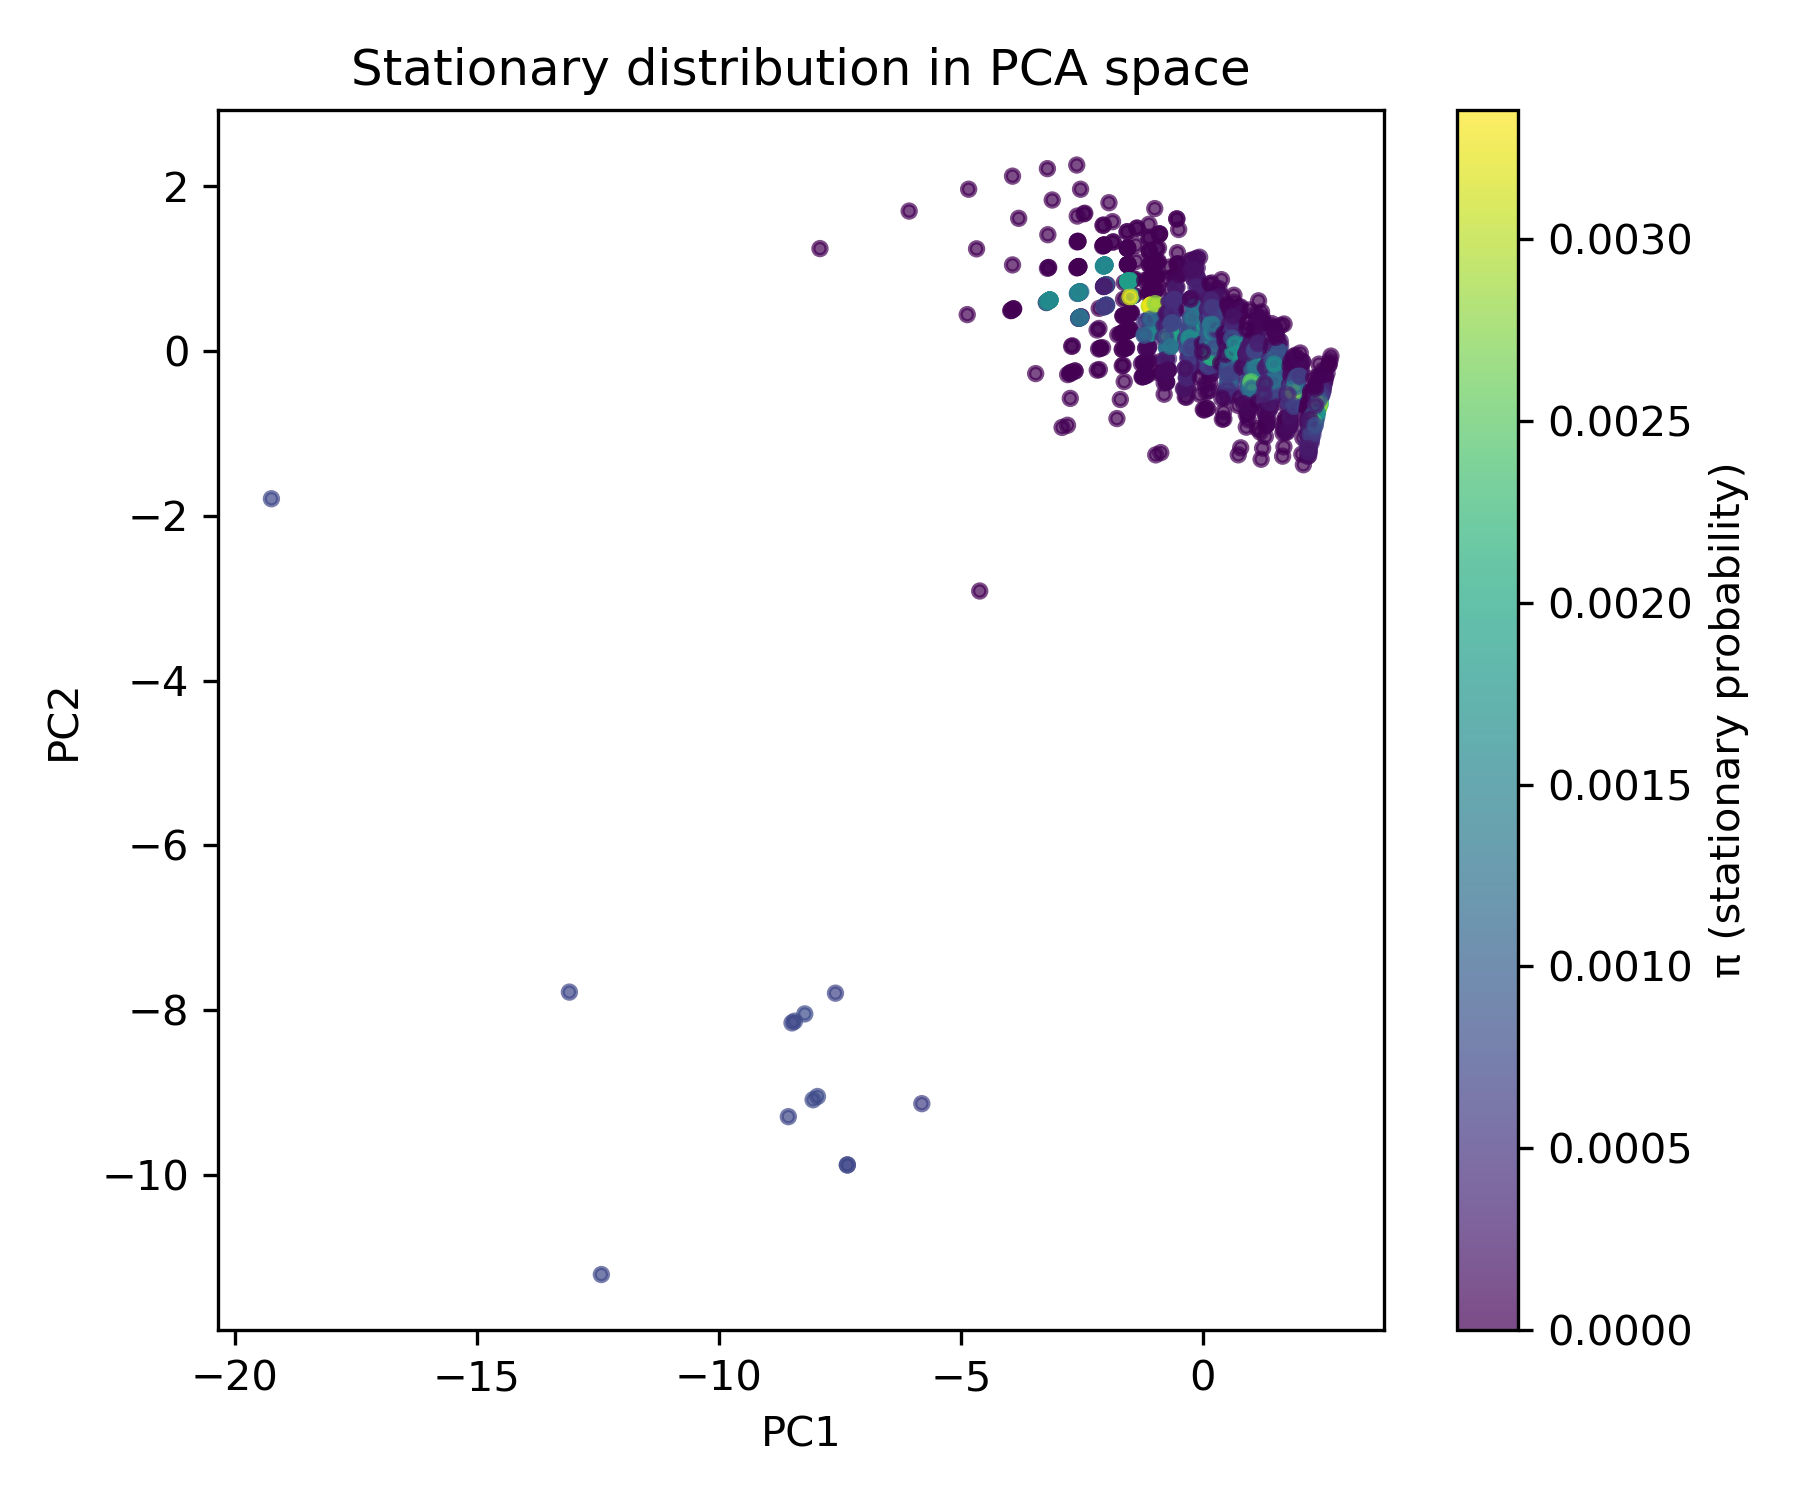
\includegraphics[width=0.7\textwidth]{figures/fig_pca_stationary.png}
\caption{Stationary distribution $\pi$ projected onto the principal components of the feature space. The nearly uniform coloring indicates that no configuration is privileged under the purely relational dynamics.}
\label{fig:stationary}
\end{figure}

\paragraph{Interpretation}
No state is privileged. The system exhibits maximal symmetry.

\section{Observers as Projections}

An observer is defined as:

\begin{equation}
O: \mathbb{R}^d \to \mathbb{R}^k
\end{equation}

with $k \ll d$.

Define:

\begin{equation}
d_O(i,j) = \|O(x_i) - O(x_j)\|
\end{equation}

Kernel:

\begin{equation}
K_O(i,j) = \exp\left(-\frac{d_O(i,j)^2}{2\sigma_O^2}\right)
\end{equation}

\subsection{Memory Coupling}

\begin{equation}
P_O = (1-\gamma)P + \gamma P_{\text{obs}}
\end{equation}

\section{Emergence of Proto-Objects}

Define:

\begin{equation}
R_O = \text{Top}_k(\pi_O)
\end{equation}

These regions correspond to stable configurations.

\begin{figure}[htbp]
\centering
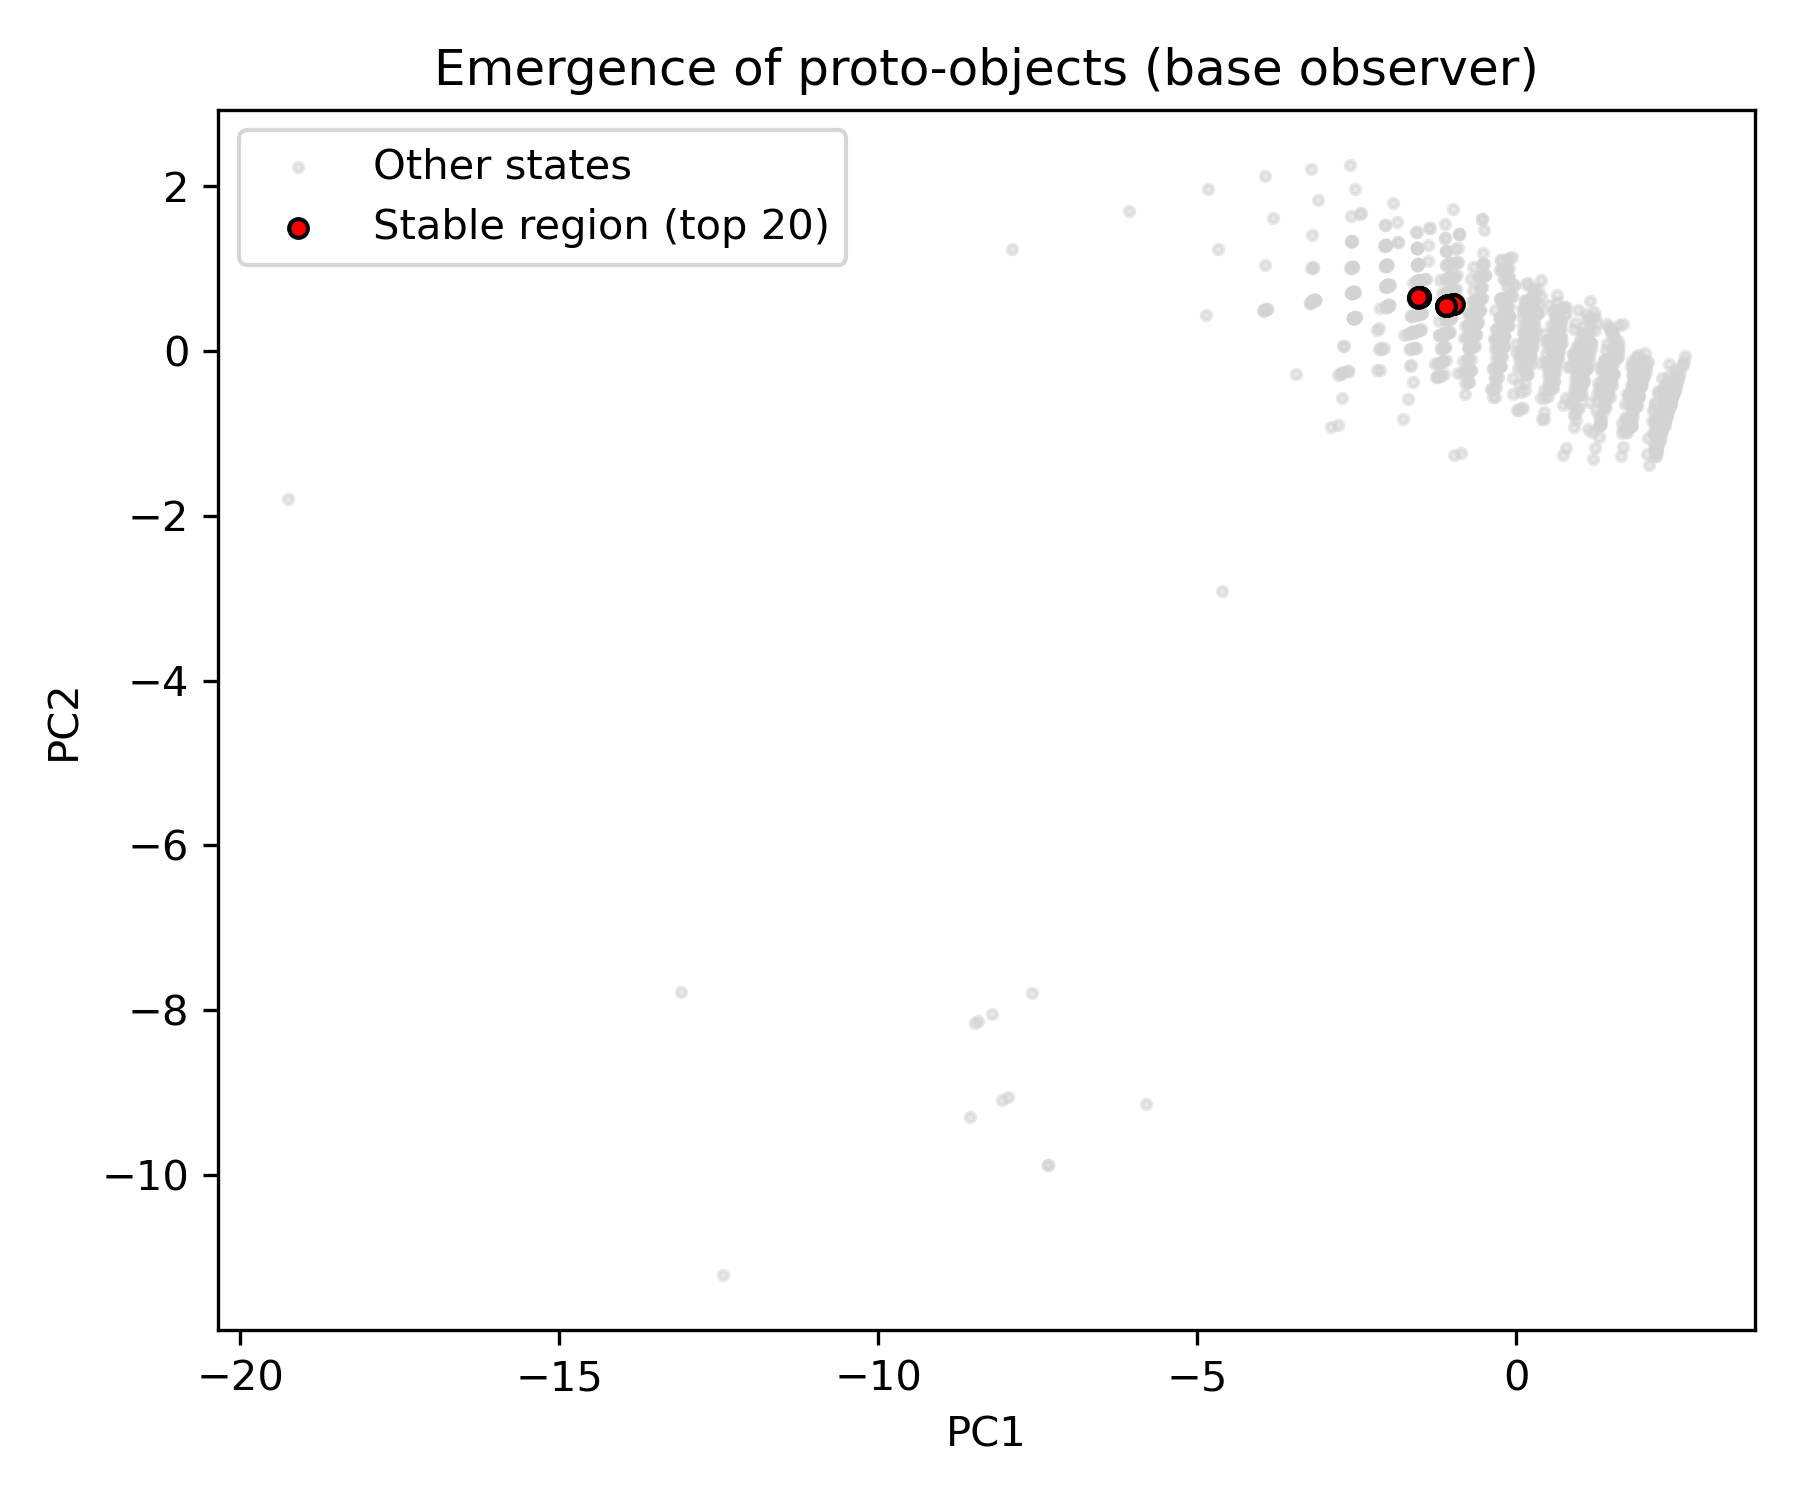
\includegraphics[width=0.7\textwidth]{figures/fig_proto_objects.png}
\caption{Projection of all states (gray) and the stable region (red) for a representative observer. The concentration in a compact area shows that the observer perceives a well-defined ``proto-object'', though it will not be shared by other observers.}
\label{fig:proto_objects}
\end{figure}

\section{Observer Dependence}

For observers $O_1, O_2$:

\begin{equation}
R_{O_1} \cap R_{O_2} \approx \emptyset
\end{equation}

Empirically:

\begin{itemize}
    \item Mean overlap $\approx 0.0369$
    \item Median overlap $= 0$
\end{itemize}

\begin{figure}[htbp]
\centering
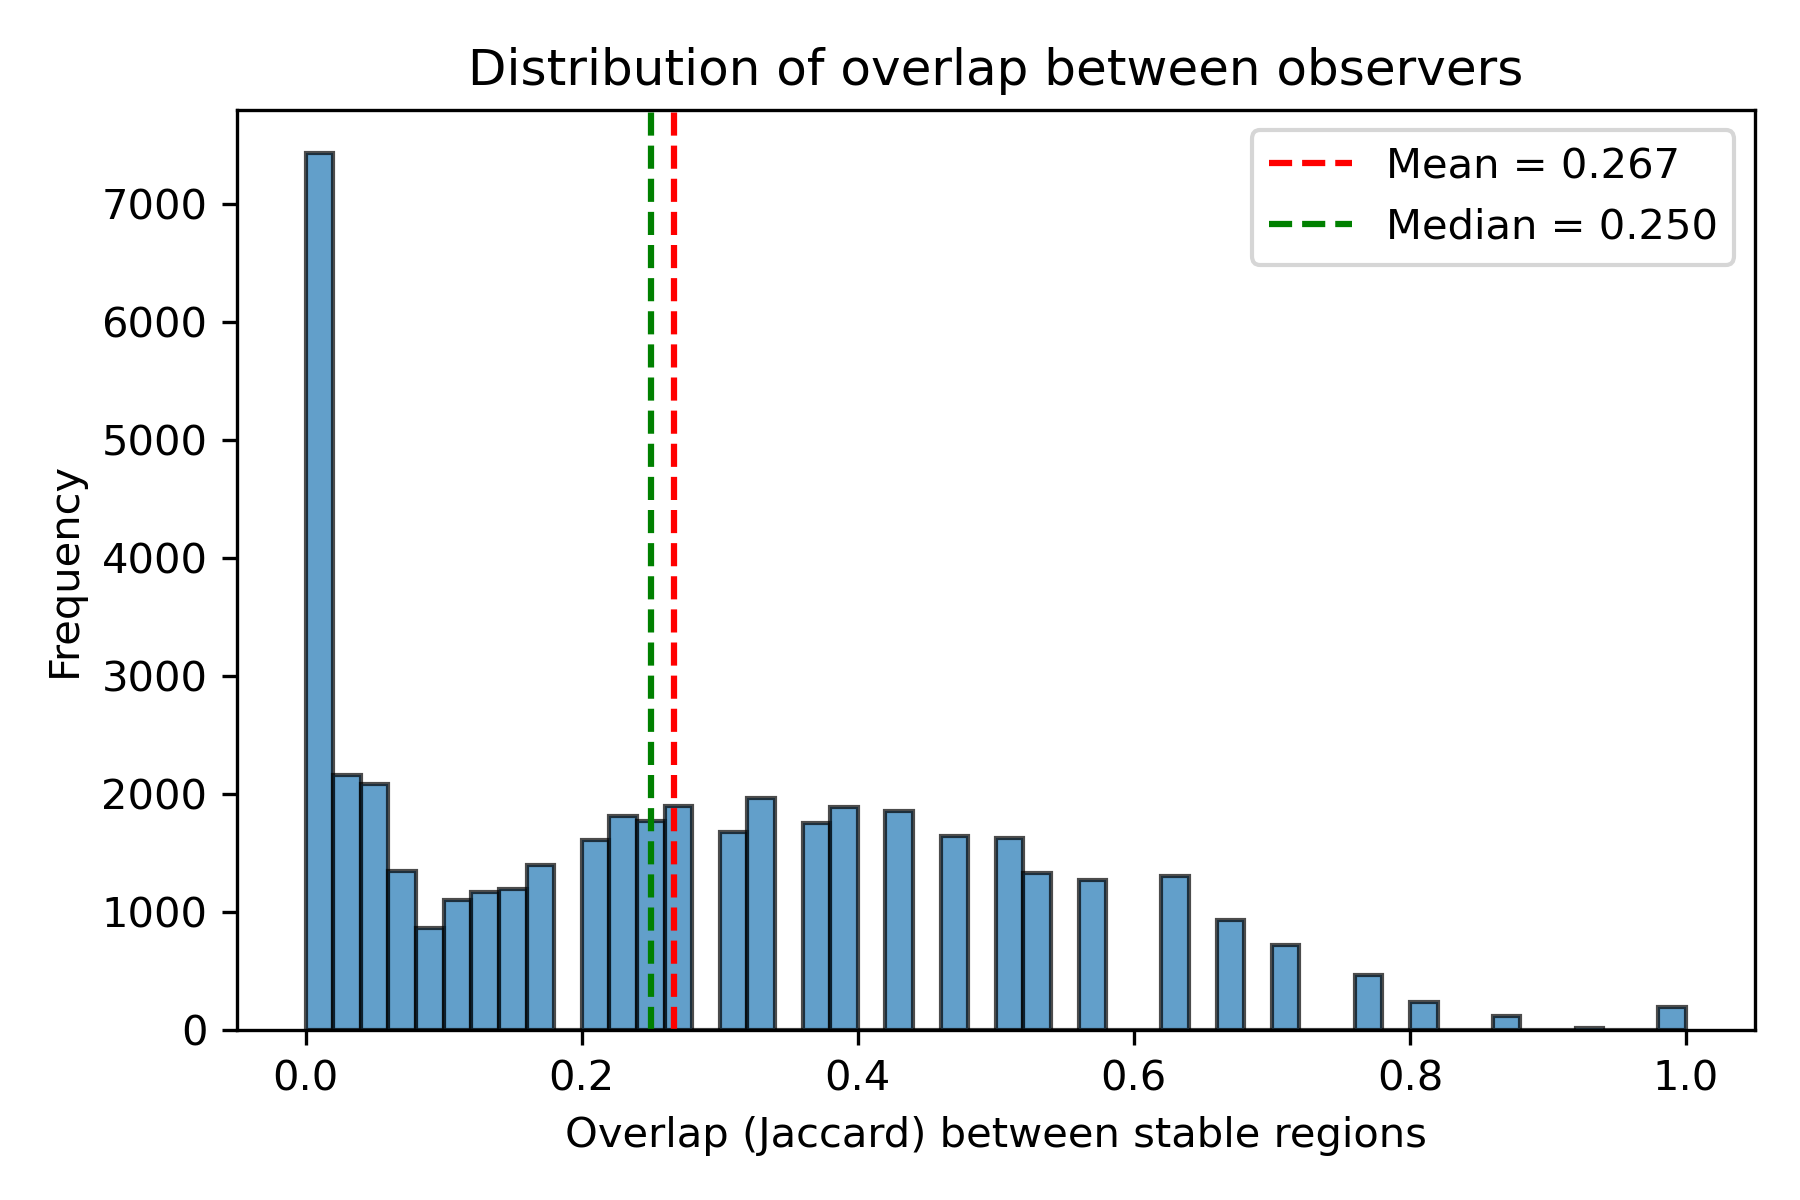
\includegraphics[width=0.7\textwidth]{figures/fig_overlap_hist.png}
\caption{Histogram of Jaccard overlaps between the stable regions of 200 randomly generated observers. The distribution is heavily concentrated near zero, confirming that different observers typically do not share a common ``reality''.}
\label{fig:overlap_hist}
\end{figure}

\section{No-Go Theorem}

\textbf{Theorem.}
There exists no non-trivial subset $S \subset \mathcal{G}$ such that:

\begin{equation}
S = R_O \quad \forall O
\end{equation}

\textbf{Proof (empirical + structural).}

Assume such $S$ exists. Then:

\begin{equation}
\forall O_1, O_2,\quad R_{O_1} = R_{O_2}
\end{equation}

But bootstrap analysis yields:

\begin{equation}
\mathbb{E}[\text{Overlap}(O_1,O_2)] \approx 0
\end{equation}

Contradiction.

This result establishes that observer-invariant objecthood cannot be recovered as a fixed point of relational dynamics.

\section{Observer Space Geometry}

Define observer graph:

\begin{equation}
O_i \sim O_j \iff \text{Overlap}(i,j) > \tau
\end{equation}

\subsection{Phase Transition}

We observe:

\begin{itemize}
    \item $\tau < 0.15$: giant component
    \item $\tau \sim 0.2$: fragmentation onset
    \item $\tau > 0.3$: isolated nodes dominate
\end{itemize}

The observed transition is analogous to percolation phenomena in random graphs \cite{percolation}.

\begin{figure}[htbp]
\centering
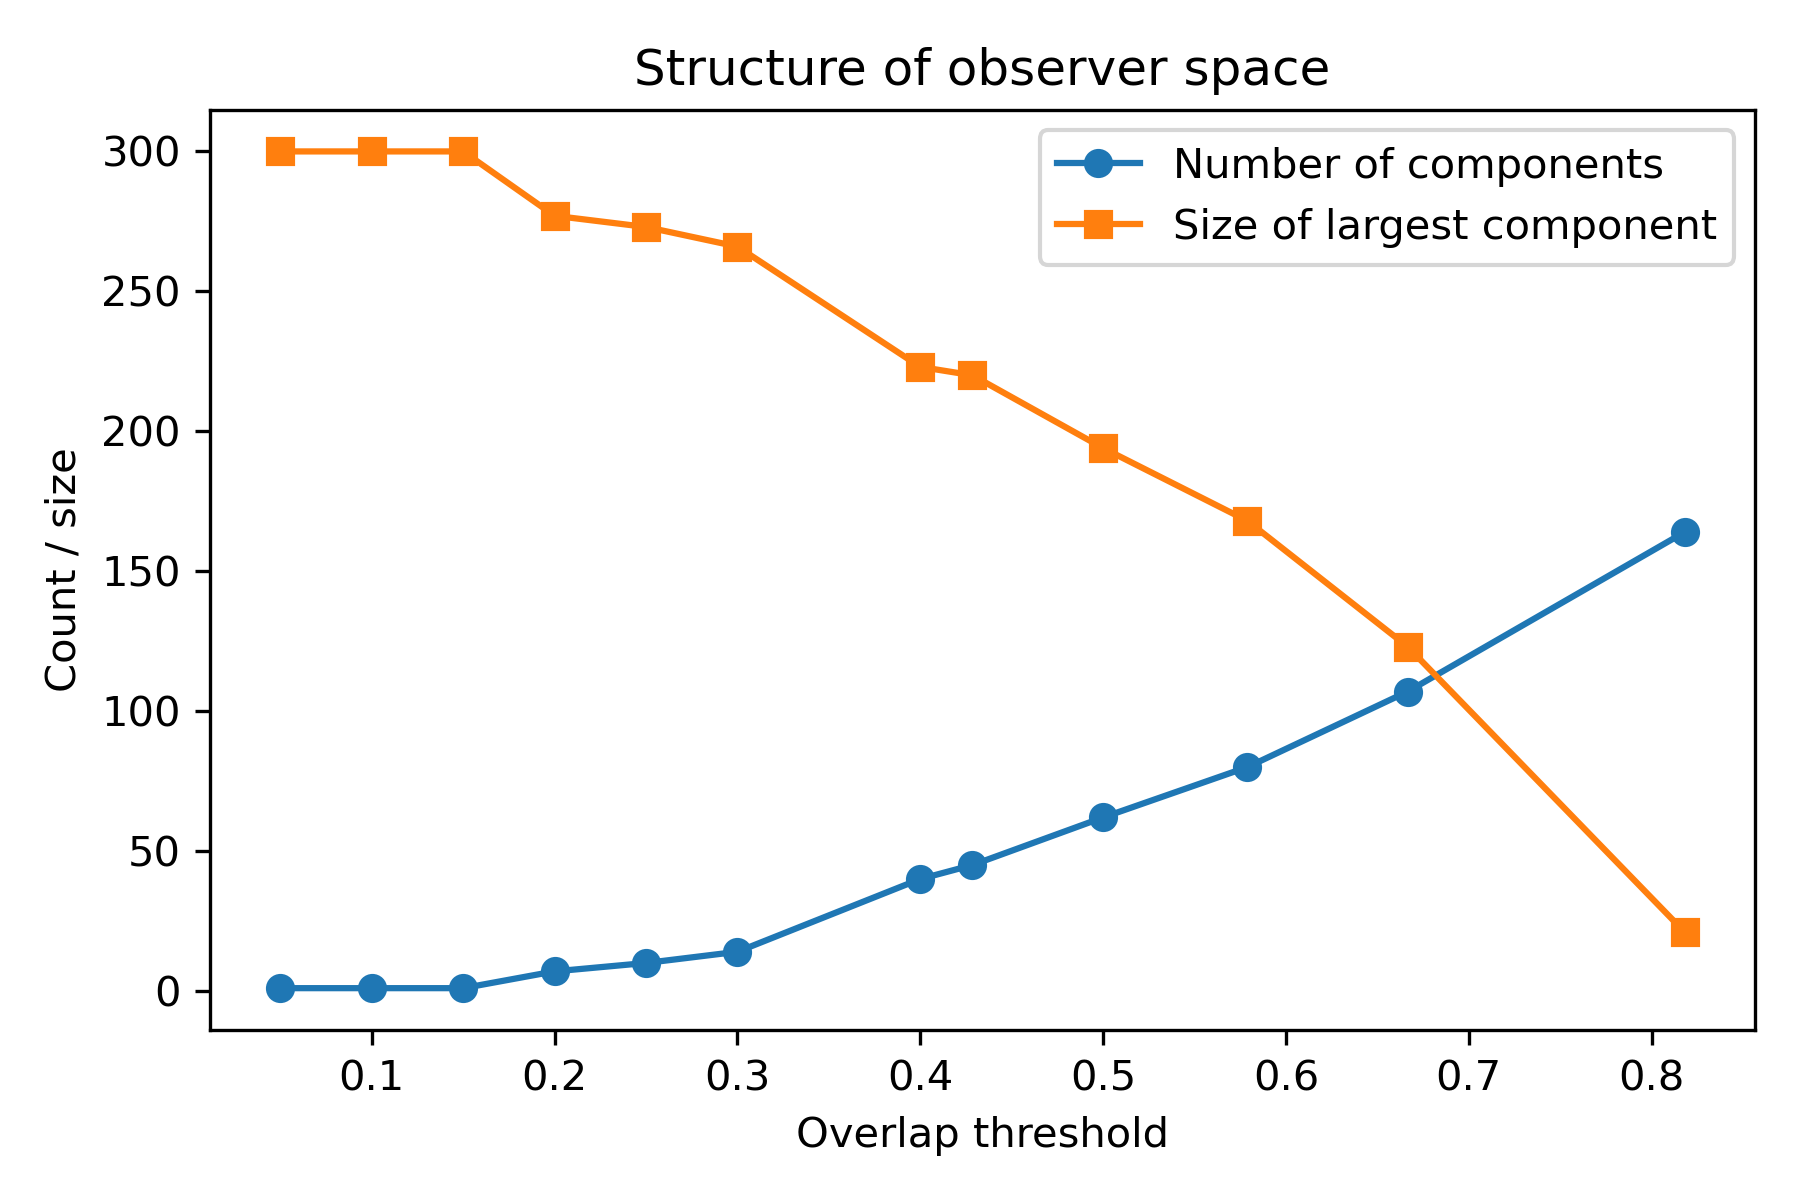
\includegraphics[width=0.7\textwidth]{figures/fig_percolation.png}
\caption{Number of components and size of the largest component in the observer graph as a function of the overlap threshold $\tau$. The transition near $\tau \approx 0.2$ indicates that observers do not organize into stable families; instead, connectivity decays rapidly.}
\label{fig:percolation}
\end{figure}

\paragraph{Interpretation}
This is analogous to percolation.

\section{Absence of Ontological Classes}

No stable partition emerges:

\begin{equation}
\mathcal{G} \neq \bigsqcup_i C_i \quad \text{(observer-invariant)}
\end{equation}

Thus, object classes are not intrinsic.

\section{Relation to Gauge and Identifiability}

The model parallels:

\begin{itemize}
    \item Gauge redundancy: multiple states, same observables
    \item Non-identifiability: parameters not uniquely determined
\end{itemize}

However, we show a stronger result:

\begin{equation}
\text{No invariant representatives exist}
\end{equation}

\section{Positioning within the Literature}

This work lies at the intersection of three domains:

\paragraph{Relational physics.}
The model is structurally aligned with relational approaches in physics, 
where states are not defined independently but through relations \cite{rovelli_relational}. 
However, unlike standard formulations, we explicitly construct a dynamical system 
in which relational structure alone fails to produce invariant objects.

\paragraph{Gauge and representational equivalence.}
Recent work has emphasized that multiple mathematical representations 
may correspond to the same physical situation \cite{weatherall}. 
Our results extend this insight: not only are representations non-unique, 
but no privileged representatives emerge even dynamically.

\paragraph{Statistical identifiability.}
In statistics, non-identifiability implies that parameters cannot be uniquely recovered from data \cite{stat_inference}. 
Here we show a stronger phenomenon: even when stable regions emerge, 
they fail to be invariant across observers, suggesting a structural limitation 
on object individuation.

\paragraph{Philosophical implications.}
While the model is not intended as a direct formalization of Madhyamaka philosophy, 
it provides a constructive analogue of its central claim: 
that apparent entities arise dependently and lack intrinsic identity \cite{nagarjuna, tsongkhapa}.
This work is also related to previous analyses that critically examined the logical assumptions of Madhyamaka reasoning from a scientific perspective \cite{madhyamaka_critique}. While those analyses questioned the universality of Madhyamaka arguments, the present work adopts a constructive approach, identifying conditions under which Madhyamaka-like conclusions emerge from relational dynamics.
\section{Reproducibility}

All figures are generated from the same dataset and codebase, ensuring reproducibility of the reported phenomena.
The full computational pipeline, including graph generation, Markov dynamics, and observer bootstrap analysis, is publicly available \cite{code_repo}.

\section{Interpretation}

We obtain:

\begin{equation}
\text{Object} = f(O, \gamma, \text{projection})
\end{equation}

Objects are:

\begin{itemize}
    \item emergent
    \item observer-dependent
    \item non-invariant
\end{itemize}

\section{Connection to Madhyamaka}

The model provides a constructive analogue of:

\begin{itemize}
    \item dependent origination
    \item absence of inherent existence
    \item failure of intrinsic identity under analysis
\end{itemize}

These results resonate with classical Madhyamaka analyses of intrinsic existence \cite{nagarjuna, tsongkhapa}.

\section{Philosophical Implications: Madhyamaka Perspective}

The results obtained in this work admit a natural interpretation in relation to classical Madhyamaka philosophy.

\paragraph{Dependent origination.}
In the model, proto-objects arise only through the interaction between relational structure and observer-dependent projections. They do not exist independently of these conditions. This mirrors the principle of dependent origination: phenomena arise only in dependence on causes, conditions, and conceptual imputation.

\paragraph{Emptiness as non-invariance.}
The absence of observer-invariant subsets provides a precise structural analogue of emptiness. In this context, emptiness does not imply non-existence, but rather the failure of any configuration to sustain identity across all observational frameworks.

\paragraph{Object of negation.}
The Madhyamaka ``object of negation'' --- an intrinsically existing entity --- corresponds, in this model, to a hypothetical subset invariant under all observers. The no-go theorem shows that no such subset exists. Thus, the object of negation can be identified with a mathematically well-defined but unrealizable structure.

\paragraph{Two truths reinterpretation.}
The model naturally supports a two-level description:
\begin{itemize}
    \item At the conventional level, proto-objects emerge and exhibit stability relative to specific observers.
    \item At the ultimate level, no observer-independent entities exist.
\end{itemize}

\paragraph{Non-reification.}
Importantly, the model does not eliminate structure or regularity. Instead, it shows that stability is relational and context-dependent. This aligns with the Madhyamaka rejection of intrinsic nature without collapsing into nihilism.

These parallels suggest that Madhyamaka conclusions can be understood as statements about the structural limitations of relational systems, rather than as purely metaphysical claims.

\section{Conclusion}

We have constructed a fully relational dynamical system in which candidate objects are represented as graph structures evolving under similarity-based Markov dynamics.

The results show that:

\begin{itemize}
    \item In the absence of observational structure, the system exhibits no privileged states.
    \item Introducing observers induces stable proto-objects.
    \item These proto-objects are robust within an observer but fail to be invariant across observers.
\end{itemize}

A no-go result establishes that no non-trivial subset of states remains invariant under all observers. Object-like structures therefore cannot be interpreted as intrinsic features of the system.

From a philosophical perspective, this provides a constructive analogue of key Madhyamaka insights:

\begin{itemize}
    \item Phenomena arise dependently on relational and observational conditions.
    \item Apparent stability does not imply intrinsic identity.
    \item The search for inherently existing objects corresponds to a mathematically well-defined but unrealizable condition.
\end{itemize}

In this framework, the ``object of negation'' is not merely a philosophical abstraction, but a precise structural impossibility: an invariant attractor that cannot exist in a relational system.

More broadly, the results suggest that objecthood should be understood as an emergent, observer-dependent phenomenon, rather than a fundamental feature of reality. This shifts the problem of ontology toward the study of relational structures, invariance, and the limits of identifiability.

The model thus bridges philosophical analysis and formal construction, showing that the absence of intrinsic existence can arise as a rigorous consequence of relational dynamics.
\section{Code and Data Availability}

All code, datasets, and scripts used to generate the results in this work are publicly available at:

\begin{center}
\url{https://github.com/eduwardus/relational-objects-paper}
\end{center}
\bibliographystyle{plain}
\bibliography{references}

\end{document}
